\Subsubsubsection{Potencia}

Para la unidad de potencia se utilizan paneles solares y una batería de gel de ciclo profundo conectados a la placa DFR0580, la cual se ocupa de cargar la batería. De esta se obtienen cuatro salidas de tensión:
\begin{itemize}
	\item Dos salidas de $5 \ V$ y $2.5 \ A$ [USB].
	\item Una salida de $5 \ V$ y $5 \ A$.
	\item Una salida de $12 \ V$ y $8 \ A$.
\end{itemize}
De estas salidas solo es necesaria aquella que posee $5 \ V$. En cuanto a la corriente, si bien es indistinto, se emplea la de $5 \ A$ para evitar problemas de falta de corriente.

\Subsubsubsection{Medición}
Para el conexionado de los sensores se diseñó una placa de soporte para la \rspi, la cual se denomina \textit{shield}. En esta se encuentra:
\begin{itemize}
	\item El módulo RTC.
	\item El acondicionamiento para la conexión de la cámara.
	\item El conexionado para el abastecimiento de energía para los sensores.
	\item Un conector para los sensores, que abarca al de humedad, temperatura, luminosidad y presencia.
	\item Un sistema de protección ante desabastecimiento de energía.
	\item Interruptores de prendido y apagado seguro.
\end{itemize}

La placa de sensores utiliza alimentación de $3.3 \ V$, la referencia de tierra, un pin GPIO para comunicación serial y el bus $I^2C$ de la \rpi. Este último se emplea para administrar la comunicación con el sensor de luminosidad y el módulo RTC, ya que ambos emplean el respectivo protocolo de comunicación del bus, en modo \textit{multi-slave}. Por otro lado, el pin serial GPIO corresponde a la comunicación del sensor de temperatura y humedad DHT-22. 
\begin{figure}[H]
	\centering
	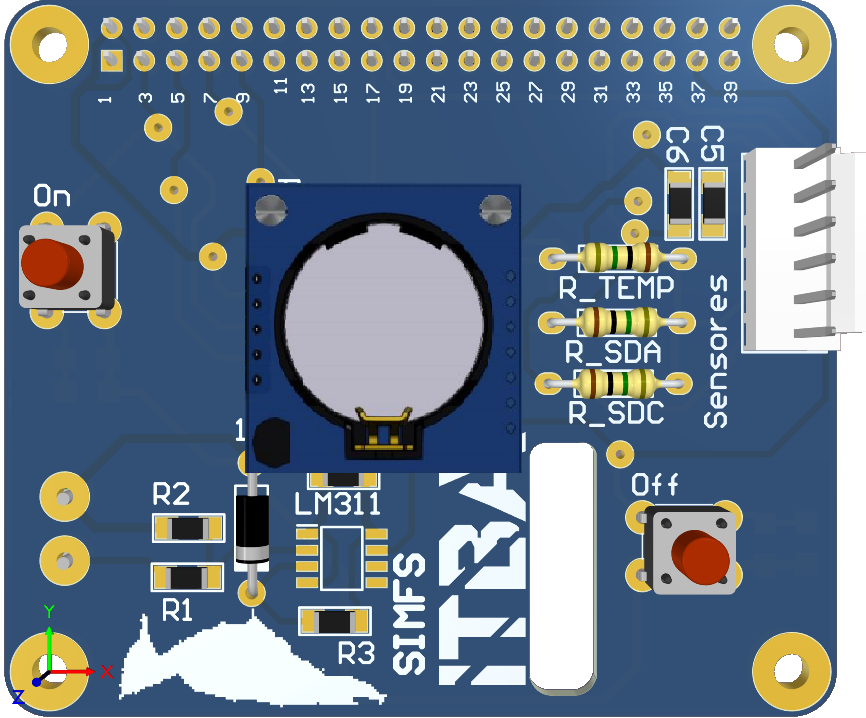
\includegraphics[width=0.75\linewidth,page=1]{ImagenesIngenieria de Detalle/shield}		
	\caption{Shield \rspi.}
	\label{fig:conexionado_Rpi}
\end{figure}

\begin{figure}[H]
	\centering
	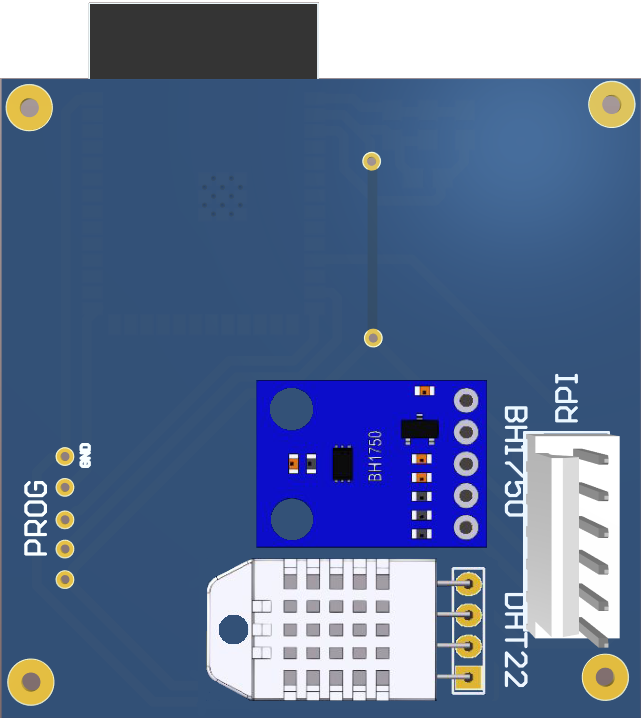
\includegraphics[width=0.75\linewidth,page=1]{ImagenesIngenieria de Detalle/sensores_top}		
	\caption{Vista \textit{top} de la placa de sensores.}
	\label{fig:sensores_top}
\end{figure}

\begin{figure}[H]
	\centering
	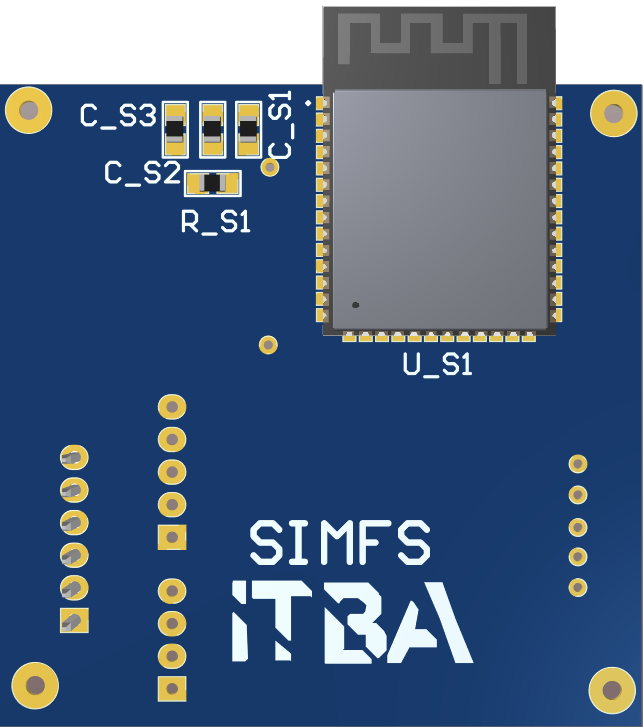
\includegraphics[width=0.75\linewidth,page=1]{ImagenesIngenieria de Detalle/sensores_bot}		
	\caption{Vista \textit{bottom} de la placa de sensores.}
	\label{fig:sensores_bottom}
\end{figure}

Por fuera del \textit{shield}, la \rspi cuenta tanto con un conector destinado al uso de una cámara como un conector mini USB por el cual se energiza la unidad. Ambos conectores se muestran en la Figura (\ref{fig:rpiFront}).
\begin{figure}[H]
	\centering
	\includegraphics[width=\linewidth,page=3]{ImagenesIngenieria de Detalle/RPI}		
	\caption{Conexionado cámara.}
	\label{fig:rpiFront}
\end{figure}

Además, cuenta con una ranura para una tarjeta SD. Esta es usada no solo para la imagen de sistema operativo, sino que también para el almacenamiento de datos.
\begin{figure}[H]
	\centering
	\includegraphics[width=0.9\linewidth,page=2]{ImagenesIngenieria de Detalle/RPI}		
	\caption{Conexionado tarjeta SD.}
	\label{fig:rpiBack}
\end{figure}
